\begin{figure}[ht]
\centering
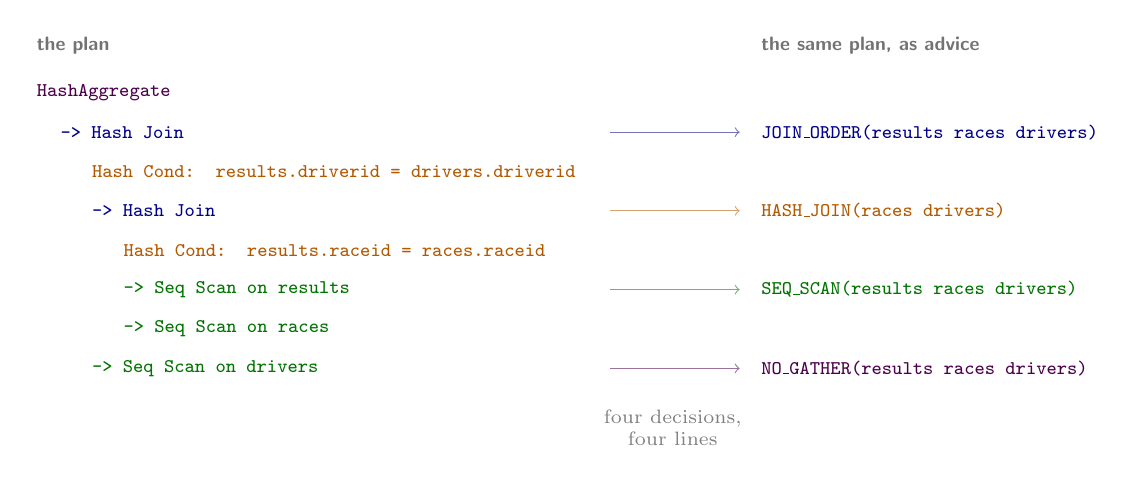
\begin{tikzpicture}[font=\small]

\colorlet{cOrder}{blue!55!black}
\colorlet{cMethod}{orange!70!black}
\colorlet{cScan}{green!45!black}
\colorlet{cPar}{violet!60!black}

\tikzset{
  node/.style   = {font=\scriptsize\ttfamily, anchor=west},
  advice/.style = {font=\scriptsize\ttfamily, anchor=west},
}

%% ---------- the plan, left ----------
\node[font=\scriptsize\bfseries\sffamily, anchor=west, black!55] at (0,4.6) {the plan};

\node[node, cPar]    at (0.0,4.0) {HashAggregate};
\node[node, cOrder]  at (0.3,3.5) {-> Hash Join};
\node[node, cMethod] at (0.7,3.0) {Hash Cond: results.driverid = drivers.driverid};
\node[node, cOrder]  at (0.7,2.5) {-> Hash Join};
\node[node, cMethod] at (1.1,2.0) {Hash Cond: results.raceid = races.raceid};
\node[node, cScan]   at (1.1,1.5) {-> Seq Scan on results};
\node[node, cScan]   at (1.1,1.0) {-> Seq Scan on races};
\node[node, cScan]   at (0.7,0.5) {-> Seq Scan on drivers};

%% ---------- the advice, right ----------
\node[font=\scriptsize\bfseries\sffamily, anchor=west, black!55] at (9.2,4.6) {the same plan, as advice};

\node[advice, cOrder]  at (9.2,3.5) {JOIN\_ORDER(results races drivers)};
\node[advice, cMethod] at (9.2,2.5) {HASH\_JOIN(races drivers)};
\node[advice, cScan]   at (9.2,1.5) {SEQ\_SCAN(results races drivers)};
\node[advice, cPar]    at (9.2,0.5) {NO\_GATHER(results races drivers)};

%% ---------- the mapping ----------
\draw[cOrder,  ->, thin, opacity=0.55] (7.4,3.5) -- (9.05,3.5);
\draw[cMethod, ->, thin, opacity=0.55] (7.4,2.5) -- (9.05,2.5);
\draw[cScan,   ->, thin, opacity=0.55] (7.4,1.5) -- (9.05,1.5);
\draw[cPar,    ->, thin, opacity=0.55] (7.4,0.5) -- (9.05,0.5);

\node[font=\scriptsize, black!50, anchor=north, align=center] at (8.2,0.1)
  {four decisions,\\four lines};

\end{tikzpicture}
\caption{\texttt{EXPLAIN (PLAN\_ADVICE)} reads the planner's choices back out as a string you can feed to the next planning cycle.}
\end{figure}
